%\section{Folded Singularities in three dimensions}
Now that we have considered the two dimensional case for a folded singularity we can extend it to a third dimension in our system. This can be done by considering a system of one fast and two slow variables \st, 
\begin{equation}
\begin{cases}
\epsilon \dot{x}&=f(x,y,z,y,\epsilon),\\
\dot{y}&=g_1(x,y,z,y,\epsilon),\\
\dot{z}&=g_2(x,y,z,y,\epsilon),
\end{cases}\label{eq: fs singularity system}
\end{equation}
which we can see is an extension of our original form - Equation \ref{SlowS} \citep{MMO}. Furthermore, \citet{MMO} also discusses that the addition of an extra slow variable causes issues with respect to the existence of a canard solution. This is because our existence ranges increases from $ O(\epsilon) $ to $ O(1) $, noting that $ \epsilon\ll 1 $ \citep{MMO}. Then for this system we are able to make similar assumptions to the previous case, Section \ref{sec:singularities-and-fold-points}, but it is obvious we now must have more than one fold point. We can see that this is the case in Figure \ref{fig: 3d folded singularity},
\begin{figure}[h!]\centering
	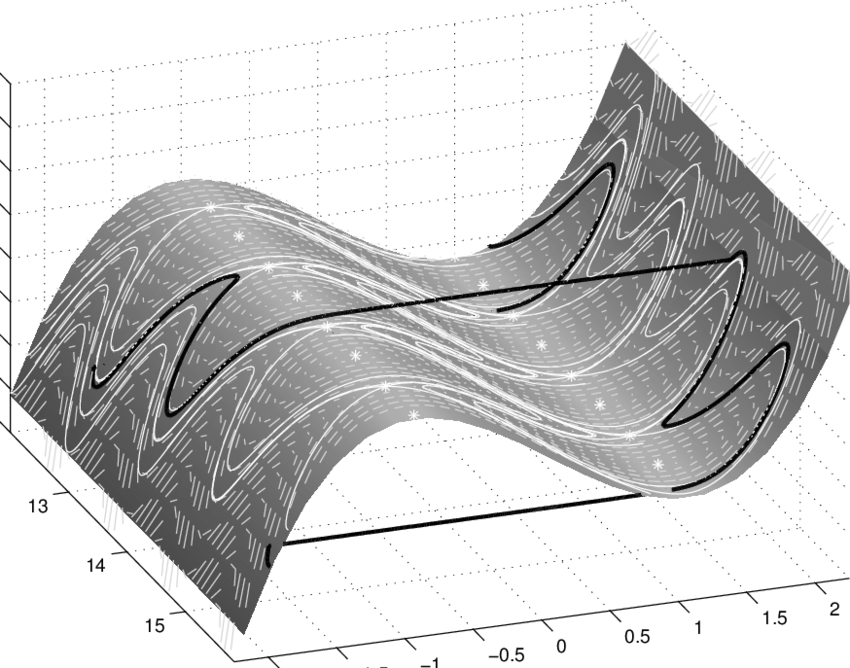
\includegraphics[height=10cm,width=14cm]{Images/Three-dimensional-plot-of-a-trajectory-for-the-van-der-Pol-equation-and-the-critical}
	\caption{Three dimensional \vdp \citep{3D-VdP}.}
	\label{fig: 3d folded singularity}
\end{figure}\newpage
as our fold point now can take multiple locations within our system. From here we are able to define some non-degeneracy conditions, much like we did in Section \ref{GSPT},
\begin{equation}
\begin{aligned}
&f(p_*,\lambda,0)=0,\\
&\pd{}{x}f(p_*,\lambda,0)=0,\\
&\pd{^2}{x^2}f(p_*,\lambda,0)\neq 0,\\
&D_{(y,z)}f(p_*,\lambda,0) \ \text{has full rank one},
\end{aligned}
\label{eq: non-degeneracy 3d system}	
\end{equation}
where we denote $ p_*=(x_*,y_*,z_*)\in F $ as our fold points and\textbf{ $ D_{(y,z)}=(\pd{f}{y},\pd{f}{z}) $ are linearly independent of one another } \citep{MMO}. In addition to this we can see from Figure \ref{fig: 3d folded singularity} that we have some interesting flows within our system. These flows do not follow the standard pattern as we saw in Figure \ref{fig: vdp flow diagram}, instead the slow flow switches its orientation when the flow hits the fold point and continue to flow in that direction, as a desingularised flow - these are called isolated singularities \citep{MMO}. %dot in diagram
As a result we are able to express these flows in the following manner, using Equation \ref{eq: non-degeneracy 3d system}, 
\begin{equation}
\begin{cases}
\dot{x}&=g_1\pd{f}{y}+g_2\pd{f}{z}\\
\dot{y}&=-g_1\pd{f}{x},\\
\dot{z}&=-g_2\pd{f}{x},
\end{cases}
\end{equation}
where we can then define a folded singularity if $ g_1(p_*,\lambda,0)\pd{}{y}f(p_*,\lambda,0)+g_2(p_*,\lambda,0)\pd{}{z}f(p_*,\lambda,0)=0 $, for our flow on branches ($ S $) \citep{MMO}. Next we need to consider the stability of our fold points. We do this by constructing the Jacobian of our system, 
\begin{equation}
J=\begin{bmatrix}
\pd{\dot{x}}{x}&\pd{\dot{x}}{y}&\pd{\dot{x}}{z}&\pd{\dot{x}}{\lambda}&\pd{\dot{x}}{\epsilon}\\
\pd{\dot{y}}{x}&\pd{\dot{y}}{y}&\pd{\dot{y}}{z}&\pd{\dot{y}}{\lambda}&\pd{\dot{y}}{\epsilon}\\
\pd{\dot{z}}{x}&\pd{\dot{z}}{y}&\pd{\dot{z}}{z}&\pd{\dot{z}}{\lambda}&\pd{\dot{z}}{\epsilon}\\
\end{bmatrix},
\end{equation}

+++Either 5x5 J with last rows zero inj extended system or just 3x3++++
which we can easily find the eigenvalues, by taking the determinant. The result of this analysis gives that we have three eigenvalues, $ \sigma_i $ for $ i=1,2,3 $ \citep{MMO}. \Wlg we can choose $ \sigma_3=0 $ because we know that at least one of our eigenvalues must be zero to account for our fold point in our system, as the \textbf{Poincar\'e diagram describes}. Then we know from standard stability theory that, at our folded singularity we will have three types of phase portrait in the form of,
\begin{equation}
\begin{cases}
Saddle \ \sigma_1\sigma_2<0: \sigma_i\in\Re,\\
Node \ \sigma_1\sigma_2>0: \sigma_i\in\Re,\\
Focus \ \sigma_1\sigma_2>0: \Im(\sigma_i)\neq 0,
\end{cases}
\end{equation}
where we can note that only our focus will have imaginary parts \citep{MMO}. \citet{MMO} illustrates this in the following Figure, 
\begin{figure}[h!]\centering
	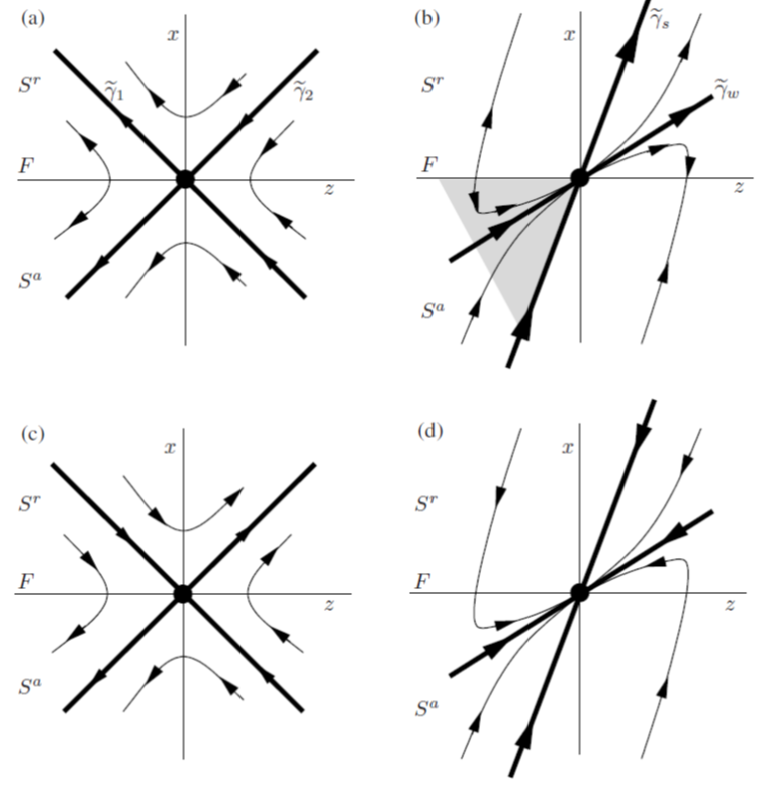
\includegraphics[height=12cm,width=12cm]{Images/foldednodesetc}
	\caption{Phase portraits of our three dimensional system where a) is a folded saddle, b) folded node, c) and d) are desingularised flows \citep{MMO}.}
	\label{fig: folded singularities}
\end{figure}\newpage%arrows switch as we have reversed time
where we can see the effect of the varying eigenvalues above. A question which is prudent to consider is, why hasn't \citep{MMO} illustrated the singular canard case for a folded focus. This is easily answered as we know that a singular canard is only present if the node or saddle connect our two connecting branches ($ S^r $ and $ S^a $). The idea that our branches are connected allows us to note that our flow is able to pass through from an attracting to a repelling manifold, which is described by Figure \ref{fig: folded singularities} \citep{CanardsinR3}. However, we find that for the focus we are unable to construct branches which connect, preventing the flow from traversing through the fold point. This idea is easily seen as we are able to note, from the imaginary eigenvalues, that there is a spiral present - Figure \ref{fig: spiral}.
\begin{figure}[h!]\centering
	\caption{The branches of a spiral}
	\label{fig: spiral}
\end{figure}\newpage
It is easily seen, from Figure \ref{fig: spiral}, that it is not possible to construct such a system that allows the flow to traverse this point. We can add further intuition to this example by considering the notion of a source (or sink), which is seen in dynamical systems and fluid mechanics. From a sink (attracting manifold) we know that our flow will always be travelling towards the singularity regardless of its starting location as described by Figure \ref{fig: spiral} meaning that is impossible to construct a repelling manifold which can connect with this singularity at the fold point - for further information see Figure \ref{fig:source-sink} in Appendix \ref{sec:definitions}. 
where we can see that we are unable to produce a system which has a singular 
\begin{theorem}[Canards in $ \Re^3 $ \citep{MMO}]\label{thm: canards in R3}
	For slow-fast systems (Equation \ref{eq: fs singularity system}) with $ \epsilon>0 $ sufficiently small the following holds:\begin{itemize} 
		\item  There are no maximal canards generated by a folded focus. For a folded saddle the two singular canards $ \bar{\gamma_{1,2}} $ perturb to maximaal canards $ \gamma_{1,2} $.
		\item  For a folded node let $\mu=\frac{\sigma_w}{\sigma_s} <1$. the singular canard $ \bar{\gamma_{s}} $ (``the strong canard'') always perturbs to a maximal canard $ \gamma_{s} $. If $ \mu^{-1}\not \in \mathbb{N} $, then the singualr canard $ \bar{\gamma_{w}} $ (``weak canard'') also perturbs to a maximal canard. We call $ \gamma_{s} $ and $ \gamma_{w} $ primary canards.
		\item For a folded node suppose $ k>0 $ is an integer such that $ 2k+1<\mu^{-1} <2k+3$ and $ \mu^-1\neq 2(k+1) $. Then, in addition to $ \gamma_{s,w} $ there are k other maximal canards, which we call secondary canard.
		\item The primary weak canard of a node undergoes a trancritical bifurcation for odd $ \mu^{-1}\in\mathbb{N} $ and a pitchfork bifurcation for even $ \mu^{-1\in\mathbb{N}} $
	\end{itemize}
	\end{theorem}
From Theorem \ref{thm: canards in R3} we have now defined the existence of a strong and weak eigenvalue \st $ |\sigma_1|>|\sigma_2| \iff |\sigma_s|>|\sigma_w| $. From this theorem we are then able to carry out explicit investigations, as we will see in Section \textbf{Not done yet} noting that a focus is a circle or sprial etc.

%desingularizing by changing the top half plane for arrows 
